\documentclass[
  aps,
  pre,
  preprint,
  longbibliography,
  floatfix
]{revtex4-2}

\usepackage[utf8]{inputenc}
\usepackage[T1]{fontenc}
\usepackage{newtxtext, newtxmath}
\usepackage[
  colorlinks=true,
  urlcolor=purple,
  citecolor=purple,
  filecolor=purple,
  linkcolor=purple
]{hyperref}
\usepackage{amsmath}
\usepackage{graphicx}
\usepackage{xcolor}
\usepackage{tikz-cd}
\usepackage[subfolder]{gnuplottex} % need to compile separately for APS

\begin{document}

\title{Smooth and global Ising universal scaling functions}

\author{Jaron Kent-Dobias}
\affiliation{Laboratoire de Physique de l'Ecole Normale Supérieure, Paris, France}

\author{James P.~Sethna}
\affiliation{Laboratory of Atomic and Solid State Physics, Cornell University, Ithaca, NY, USA}

\date\today

\begin{abstract}
\end{abstract}

\maketitle

At continuous phase transitions the thermodynamic properties of physical
systems have singularities. Celebrated renormalization group analyses imply
that not only the principal divergence but entire functions are
\emph{universal}, meaning that they will appear at any critical points that
connect phases of the same symmetries in the same spatial dimension. The study
of these universal functions is therefore doubly fruitful: it provides both a
description of the physical or model system at hand, and \emph{every other
system} whose symmetries, interaction range, and dimension puts it in the same
universality class.

The continuous phase transition in the two-dimensional Ising model is the most
well studied, and its universal thermodynamic functions have likewise received
the most attention. Precision numeric work both on the lattice critical theory
and on the ``Ising'' conformal field theory (related by universality) have
yielded high-order polynomial expansions of those functions, along with a
comprehensive understanding of their analytic properties
\cite{Fonseca_2003_Ising, Mangazeev_2008_Variational, Mangazeev_2010_Scaling}.
In parallel, smooth approximations of the Ising ``equation of state'' produce
convenient, evaluable, differentiable empirical functions
\cite{Caselle_2001_The}. Despite being differentiable, these approximations
become increasingly poor when derivatives are taken due to the absence of
subtle singularities.

This paper attempts to find the best of both worlds: a smooth approximate
universal thermodynamic function that respects the global analyticity of the
Ising free energy. First, parametric coordinates are introduced that remove unnecessary
singularities from the scaling function. Then the arbitrary analytic
functions that compose those coordinates are approximated by truncated
polynomials whose coefficients are fixed by matching the series expansions of
the universal function.

\section{Universal scaling functions}

A renormalization group analysis predicts that certain thermodynamic functions
will be universal in the vicinity of any critical point in the Ising
universality class. Here we will explain precisely what is meant by universal.

Suppose one controls a temperature-like parameter $T$ and a magnetic field-like
parameter $H$, which in the proximity of a critical point at $T=T_c$ and $H=0$
have normalized reduced forms $t=(T-T_c)/T_c$ and $h=H/T$. Thermodynamic
functions are derived from the free energy per site $f$, which depends on $t$
and $h$. Renormalization group analysis can be used calculated the flow of
these parameters under continuous changes of scale, yielding flow equations of
the form
\begin{align} \label{eq:raw.flow}
  \frac{dt}{d\ell}=\frac1\nu t+\cdots
  &&
  \frac{dh}{d\ell}=\frac{\beta\delta}\nu h+\cdots
  &&
  \frac{df}{d\ell}=Df+\cdots
\end{align}
where $D$ is the dimension of space and $\nu$, $\beta$, and $\delta$ are
dimensionless constants. The flow equations are truncated here, but in general
all terms allowed by symmetry are present on their righthand side. By making a
near-identity transformation to the coordinates and the free energy of the form
$u_t(t, h)=t+\cdots$, $u_h(t, h)=h+\cdots$, and $u_f(f,t,h)=f+\cdots$, one can
bring the flow equations into an agreed upon simplest normal form
\begin{align} \label{eq:flow}
  \frac{du_t}{d\ell}=\frac1\nu u_t
  &&
  \frac{du_h}{d\ell}=\frac{\beta\delta}\nu u_h
  &&
  \frac{du_f}{d\ell}=Du_f-\frac1{4\pi}u_t^2
\end{align}
which are exact as written \cite{Raju_2019_Normal}. The flow of the parameters
is made exactly linear, while that of the free energy is linearized as nearly
as possible. The quadratic term in that equation is unremovable due to a
resonance between the value of $\nu$ and the spatial dimension in two
dimensions, while its coefficient is chosen as a matter of convention. Solving
these equations for $u_f$ yields
\begin{equation}
  \begin{aligned}
    u_f(u_t, u_h)
    &=|u_t|^{D\nu}\mathcal F_\pm(u_h|u_t|^{-\beta\delta})+\frac{|u_t|^{D\nu}}{8\pi}\log u_t^2 \\
    &=|u_h|^{D\nu/\beta\delta}\mathcal F_0(u_t|u_h|^{-1/\beta\delta})+\frac{|u_t|^{D\nu}}{8\pi}\log u_h^{2/\beta\delta} \\
  \end{aligned}
\end{equation}
where $\mathcal F_\pm$ and $\mathcal F_0$ are undetermined scaling functions.
The scaling functions are universal in the sense that if another system whose
critical point belongs to the same universality class has its parameters
brought to the form \eqref{eq:flow}, one will see the same functional form (up
to constant rescaling of $u_t$ and $u_h$).

The analyticity of the free energy at finite size implies that the functions
$\mathcal F_\pm$ and $\mathcal F_0$ have power-law expansions of their
arguments about zero. This is not the case at infinity: since $\mathcal
F_0(\eta)=\eta^{D\nu}\mathcal F_\pm(\eta^{-1/\beta\delta})$ has
a power-law expansion about zero, $\mathcal F_\pm(\xi)\sim
\xi^{D\nu/\beta\delta}$ for large $\xi$.


For the scale of $u_t$ and $u_h$, we adopt the same convention as used by
\cite{Fonseca_2003_Ising}. The dependence of the nonlinear scaling variables on
the parameters $t$ and $h$ is system-dependent, and their form can be found for
common model systems (the square- and triangular-lattice Ising models) in the
literature \cite{Mangazeev_2010_Scaling, Clement_2019_Respect}.
To connect with Mangazeev and Fonseca, $\mathcal F_0(x)=\tilde\Phi(-x)=\Phi(-x)+(x^2/8\pi) \log x^2$ and $\mathcal F_\pm(x)=G_{\mathrm{high}/\mathrm{low}}(x)$.


\section{Singularities}

\subsection{Essential singularity at the abrupt transition}

In the low temperature phase, the free energy as a function of field has an
essential singularity at zero field, which becomes a branch cut along the
negative-$h$ axis when analytically continued to negative $h$
\cite{Langer_1967_Theory}. The origin can be schematically understood to arise
from a singularity that exists in the complex free energy of the metastable
phase of the model, suitably continued into the equilibrium phase. When the
equilibrium Ising model with positive magnetization is subjected to a small
negative magnetic field, its equilibrium state instantly becomes one with a
negative magnetization. However, under physical dynamics it takes time to
arrive at this state, which happens after a fluctuation containing a
sufficiently large equilibrium `bubble' occurs.

The bulk of such a bubble of radius $R$ lowers the free energy by
$2M|H|V_DR^D$, where $D$ is the dimension of space, $M$ is the magnetization,
$H$ is the external field, and $V_D$ is the volume of a $D$-ball, but its
surface raises the free energy by $\sigma S_DR^{D-1}$, where $\sigma$ is the
surface tension between the stable--metastable interface and $S_D$ is the
volume of a $(D-1)$-sphere. The bubble is sufficiently large to decay
metastable state when the differential bulk savings outweigh the surface costs.

This critical bubble occurs with free energy cost
\begin{equation}
  \begin{aligned}
    \Delta F_c
      &\simeq\left(\frac{S_D\sigma}D\right)^D\left(\frac{D-1}{2V_DM|H|}\right)^{D-1} \\
      &\simeq T\left(\frac{S_D\mathcal S(0)}D\right)^D\left[\frac{2V_D\mathcal M(0)}{D-1}ht^{-\beta\delta}\right]^{-(D-1)}
  \end{aligned}
\end{equation}
where $\mathcal S(0)$ and $\mathcal M(0)$ are the critical amplitudes for the
surface tension and magnetization, respectively \textbf{[find more standard
notation]} \cite{Kent-Dobias_2020_Novel}.
In the context of statistical mechanics, Langer demonstrated that the decay rate is asymptotically proportional to the imaginary part of the free energy in the metastable phase, with (assuming Arrhenius behavior)
\begin{equation}
  \operatorname{Im}f\propto\Gamma\sim e^{-\beta\Delta F_c}=e^{-1/(\tilde B|h||t|^{-\beta\delta})^{D-1}}
\end{equation}
which can be more rigorously related in the context of quantum field theory [ref?].

\begin{figure}
  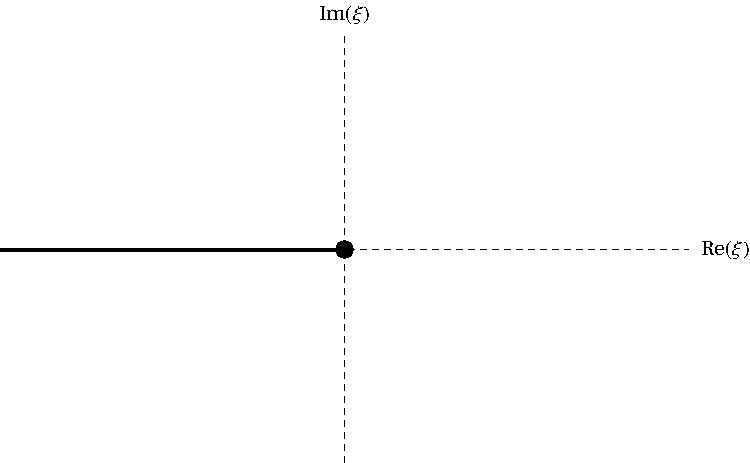
\includegraphics{figs/F_lower_singularities.pdf}
  \caption{
    Analytic structure of the low-temperature scaling function $\mathcal F_-$
    in the complex $\xi=u_h|u_t|^{-\beta\delta}\propto H$ plane. The circle
    depicts the essential singularity at the first order transition, while the
    solid line depicts Langer's branch cut.
  } \label{fig:lower.singularities}
\end{figure}
  
This is a singular contribution that depends principally on the scaling
invariant $ht^{-\beta\delta}\simeq u_h|u_t|^{-\beta\delta}$. It is therefore
suggestive that this should be considered a part of the singular free energy
$f_s$, and moreover part of the scaling function that composes it. We will
therefore make the ansatz that
\begin{equation} \label{eq:essential.singularity}
  \operatorname{Im}\mathcal F_-(\xi)=A\Theta(-\xi)|\xi|^{-b}e^{-1/(\tilde B|\xi|)^{d-1}}\left(1+O(\xi)\right)
\end{equation}
\cite{Houghton_1980_The}
The exponent $b$ depends on dimension and can be found through a more careful
accounting of the entropy of long-wavelength fluctuations in the droplet
surface, and in two dimensions $b=-1$ \cite{Gunther_1980_Goldstone}.

\subsection{Yang--Lee edge singularity}

At finite size, the Ising model free energy is an analytic function of
temperature and field because it is the logarithm of a sum of positive analytic
functions. However, it can and does have singularities in the complex plane due
to zeros of the partition function at complex argument, and in particular at
imaginary values of field, $h$. Yang and Lee showed that in the thermodynamic
limit of the high temperature phase of the model, these zeros form a branch cut
along the imaginary $h$ axis that extends to $\pm i\infty$ starting at the
point $\pm ih_{\mathrm{YL}}$ \cite{Yang_1952_Statistical, Lee_1952_Statistical}.
The singularity of the phase transition occurs because these branch cuts
descend and touch the real axis as $T$ approaches $T_c$, with
$h_{\mathrm{YL}}\propto t^{\beta\delta}$. This implies that the
high-temperature scaling function for the Ising model should have complex
branch cuts beginning at $\pm i\xi_{\mathrm{YL}}$ for a universal constant
$\xi_{\mathrm{YL}}$.

\begin{figure}
  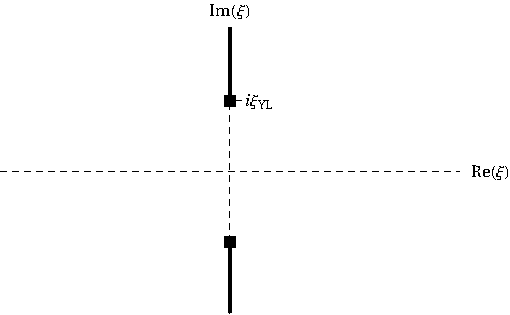
\includegraphics{figs/F_higher_singularities.pdf}
  \caption{
    Analytic structure of the high-temperature scaling function $\mathcal F_+$
    in the complex $\xi=u_h|u_t|^{-\beta\delta}\propto H$ plane. The squares
    depict the Yang--Lee edge singularities, while the solid lines depict
    branch cuts.
  } \label{fig:higher.singularities}
\end{figure}

The Yang--Lee singularities are critical points in their own right, with their own universality class different from that of the Ising model \cite{Fisher_1978_Yang-Lee}.

\begin{equation}
  \mathcal F_+(\xi)
  =A(\xi) +B(\xi)[1+(\xi/\xi_{\mathrm{YL}})^2]^{1+\sigma}+C(\xi)+\cdots
\end{equation}
for edge exponent $\sigma$.

\cite{Cardy_1985_Conformal}
\cite{Connelly_2020_Universal}
\cite{An_2016_Functional}
\cite{Zambelli_2017_Lee-Yang}
\cite{Gliozzi_2014_Critical}

\section{Parametric coordinates}

The invariant combinations $u_h|u_t|^{-\beta\delta}$ or
$u_t|u_h|^{-1/\beta\delta}$ are natural variables to describe the scaling
functions, but prove unwieldy when attempting to make smooth approximations.
This is because, when defined in terms of these variables, scaling functions
that have polynomial expansions at small argument have nonpolynomial expansions
at large argument. Rather than deal with the creative challenge of dreaming up
functions with different asymptotic expansions in different limits, we adopt
different coordinates, in terms of which a scaling function can be defined that
has polynomial expansions in \emph{all} limits.

In all dimensions, the Schofield coordinates $R$ and $\theta$ will be implicitly defined by
\begin{align} \label{eq:schofield}
  u_t(R, \theta) = Rt(\theta)
  &&
  u_h(R, \theta) = R^{\beta\delta}h(\theta)
\end{align}
where $t$ and $h$ are polynomial functions selected so as to associate different scaling limits with different values of $\theta$. We will adopt standard forms for these functions, given by
\begin{align} \label{eq:schofield.funcs}
  t(\theta)=1-\theta^2
  &&
  h(\theta)=\left(1-\frac{\theta^2}{\theta_c^2}\right)\sum_{i=0}^\infty h_i\theta^{2i+1}
\end{align}
This means that $\theta=0$ corresponds to the high-temperature zero-field line,
$\theta=1$ to the critical isotherm at nonzero field, and $\theta=\theta_c$ to
the low-temperature zero-field (phase coexistence) line.

In practice the infinite series in \eqref{eq:schofield.funcs} cannot be
entirely fixed, and it will be truncated at finite order. We will notate the
truncation an upper bound of $n$ by $h^{(n)}$. The convergence of the
coefficients as $n$ is increased will be part of our assessment of the success
of the convergence of the scaling form.

One can now see the convenience of these coordinates. Both scaling variables depend only on $\theta$, as
\begin{align}
  \xi&=u_h|u_t|^{-\beta\delta}=h(\theta)|t(\theta)|^{-\beta\delta} \\
  \eta&=u_t|u_h|^{-1/\beta\delta}=t(\theta)|h(\theta)|^{-1/\beta\delta}.
\end{align}
Moreover, both scaling variables have polynomial expansions in $\theta$ near zero, with
\begin{align}
  &\xi= h'(0)|t(0)|^{-\beta\delta}\theta+\cdots  && \text{for $\theta\simeq0$}\\
  &\xi=h'(\theta_c)|t(\theta_c)|^{-\beta\delta}(\theta-\theta_c)+\cdots && \text{for $\theta\simeq\theta_c$}
  \\
  &\eta=-2(\theta-1)h(1)^{-1/\beta\delta}+\cdots && \text{for $\theta\simeq1$}.
\end{align}
Since the scaling functions $\mathcal F_\pm(\xi)$ and $\mathcal F_0(\eta)$ have
polynomial expansions about small $\xi$ and $\eta$, respectively, this implies
both will have polynomial expansions in $\theta$ at all three places above.

Therefore, in Schofield coordinates one expects to be able to define a global
scaling function $\mathcal F(\theta)$ which has a polynomial expansion in its
argument for all real $\theta$ by
\begin{equation}
  u_f(R,\theta)=R^{D\nu}\mathcal F(\theta)+t(\theta)^2\frac{R^2}{8\pi}\log R^2
\end{equation}
For small $\theta$, $\mathcal F(\theta)$ will
resemble $\mathcal F_+$, for $\theta$ near one it will resemble $\mathcal F_0$,
and for $\theta$ near $\theta_c$ it will resemble $\mathcal F_-$. This can be seen explicitly using the definitions \eqref{eq:schofield} to relate the above form to the original scaling functions, giving
\begin{equation} \label{eq:scaling.function.equivalences.2d}
  \begin{aligned}
    \mathcal F(\theta)
    &=|t(\theta)|^{D\nu}\mathcal F_\pm\left[h(\theta)|t(\theta)|^{-\beta\delta}\right]
    +\frac{t(\theta)^2}{8\pi}\log t(\theta)^2\\
    &=|h(\theta)|^{D\nu/\beta\delta}\mathcal F_0\left[t(\theta)|h(\theta)|^{-1/\beta\delta}\right]
    +\frac{t(\theta)^2}{8\pi}\log h(\theta)^{2/\beta\delta}
  \end{aligned}
\end{equation}
This leads us
to expect that the singularities present in these functions will likewise be
present in $\mathcal F(\theta)$. This is shown in Figure
\ref{fig:schofield.singularities}. Two copies of the Langer branch cut stretch
out from $\pm\theta_c$, where the equilibrium phase ends, and the Yang--Lee
edge singularities are present on the imaginary-$\theta$ line, where they must be since $\mathcal F$ has the same symmetry in $\theta$ as $\mathcal F_+$ has in $\xi$.

The location of the Yang--Lee edge singularities can be calculated directly from the coordinate transformation \eqref{eq:schofield}. Since $h(\theta)$ is an odd real polynomial for real $\theta$, it is imaginary for imaginary $\theta$. Therefore, one requires that
\begin{equation}
  i\xi_{\mathrm{YL}}=\frac{h(i\theta_{\mathrm{YL}})}{(1+\theta_{\mathrm{YL}}^2)^{-\beta\delta}}
\end{equation}
The location $\theta_c$ is not fixed by any principle and will be left a floating parameter.

\begin{figure}
  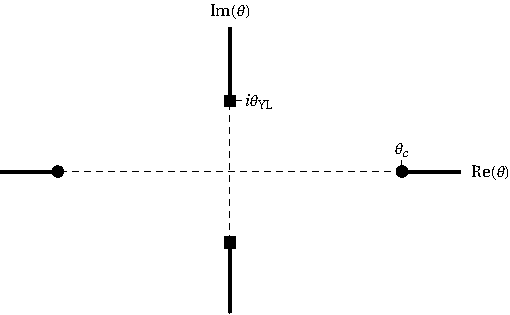
\includegraphics{figs/F_theta_singularities.pdf}
  \caption{
    Analytic structure of the global scaling function $\mathcal F$ in the
    complex $\theta$ plane. The circles depict essential singularities of the
    first order transitions, the squares the Yang--Lee singularities, and the
    solid lines depict branch cuts.
  } \label{fig:schofield.singularities}
\end{figure}

\subsection{Functional form for the parametric free energy}

As we have seen in the previous sections, the unavoidable singularities in the
scaling functions are readily expressed as singular functions in the imaginary
part of the free energy.

Our strategy follows. First, we take the known singular expansions of the imaginary parts of the scaling functions $\mathcal F_{\pm}(\xi)$ and produce simplest form accessible under polynomial coordinate changes of $\xi$. Second, we assert that the imaginary part of $\mathcal F(\theta)$ must have this simplest form. Third, we perform a Kramers--Kronig type transformation to establish an explicit form for the real part of $\mathcal F(\theta)$. Finally, we make good on the assertion posited in the second step by fixing the Schofield coordinate transformation to produce the correct coefficients known for the real part of $\mathcal F_{\pm}$.

This success of this stems from the commutative diagram below. So long as the
application of Schofield coordinates and the dispersion relation can be said to
commute, we may assume we have found correct coordinates for the simplest form
of the imaginary part to be fixed in reality by the real part.
\[
  \begin{tikzcd}[row sep=large, column sep = 9em]
  \operatorname{Im}\mathcal F_\pm(\xi) \arrow{r}{\text{Kramers--Kronig in $\xi$}} \arrow[]{d}{\text{Schofield}} & \operatorname{Re}\mathcal F_{\pm}(\xi) \arrow{d}{\text{Schofield}} \\%
  \operatorname{Im}\mathcal F(\theta) \arrow{r}{\text{Kramers--Kronig in $\theta$}}& \operatorname{Re}\mathcal F(\theta)
\end{tikzcd}
\]

\begin{figure}
  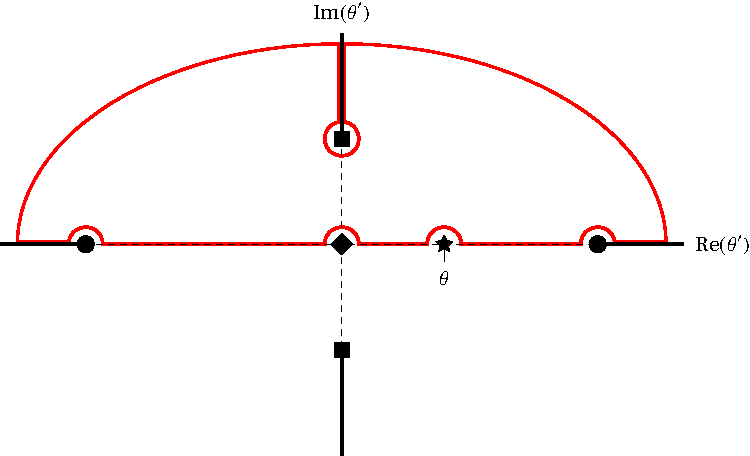
\includegraphics{figs/contour_path.pdf}
  \caption{
    Integration contour over the global scaling function $\mathcal F$ in the
    complex $\theta$ plane used to produce the dispersion relation. The
    circular arc is taken to infinity, while the circles around the
    singularities are taken to zero.
  } \label{fig:contour}
\end{figure}

As $\theta\to\infty$, $\mathcal F(\theta)\sim\theta^{2/\beta\delta}$. In order that the contribution from the arc of the contour vanish, we must have the integrand vanish sufficiently fast at infinity. Since $2/\beta\delta<2$ in all dimensions, we will simply use 2.
\begin{equation}
  0=\oint_{\mathcal C}d\vartheta\,\frac{\mathcal F(\vartheta)}{\vartheta^2(\vartheta-\theta)}
\end{equation}
where $\mathcal C$ is the contour in Figure \ref{fig:contour}. The only
nonvanishing contributions from this contour are along the real line and along
the branch cut in the upper half plane. For the latter contributions, the real
parts of the integration up and down cancel out, while the imaginary part
doubles. This gives
\begin{equation}
  \begin{aligned}
    0&=\left[\int_{-\infty}^\infty+\lim_{\epsilon\to0}\left(\int_{i\infty-\epsilon}^{i\theta_{\mathrm{YL}}-\epsilon}+\int^{i\infty+\epsilon}_{i\theta_{\mathrm{YL}}+\epsilon}\right)\right]
      d\vartheta\,\frac{\mathcal F(\vartheta)}{\vartheta^2(\vartheta-\theta)} \\
     &=\int_{-\infty}^\infty d\vartheta\,\frac{\mathcal F(\vartheta)}{\vartheta^2(\vartheta-\theta)}
     +2i\int_{i\theta_{\mathrm{YL}}}^{i\infty}d\theta'\,\frac{\operatorname{Im}\mathcal F(\vartheta)}{\vartheta^2(\vartheta-\theta)} \\
     &=-i\pi\frac{\mathcal F(\theta)}{\theta^2}+\mathcal P\int_{-\infty}^\infty d\vartheta\,\frac{\mathcal F(\vartheta)}{\vartheta^2(\vartheta-\theta)}
     +2i\int_{i\theta_{\mathrm{YL}}}^{i\infty}d\vartheta\,\frac{\operatorname{Im}\mathcal F(\vartheta)}{\vartheta^2(\vartheta-\theta)}
  \end{aligned}
\end{equation}
In principle one would need to account for the residue of the pole at zero, but since its order is less than two and $\mathcal F(0)=\mathcal F'(0)=0$, this evaluates to zero.
\begin{equation}
  \mathcal F(\theta)
  =\frac{\theta^2}{i\pi}\mathcal P\int_{-\infty}^\infty d\vartheta\,\frac{\mathcal F(\vartheta)}{\vartheta^2(\vartheta-\theta)}
  +\frac{2\theta^2}\pi\int_{i\theta_{\mathrm{YL}}}^{i\infty}d\vartheta\,\frac{\operatorname{Im}\mathcal F(\theta')}{\vartheta^2(\vartheta-\theta)}
\end{equation}
\begin{equation}
  \operatorname{Re}\mathcal F(\theta)
  =\frac{\theta^2}{\pi}\mathcal P\int_{-\infty}^\infty d\vartheta\,\frac{\operatorname{Im}\mathcal F(\vartheta)}{\vartheta^2(\vartheta-\theta)}
  -\frac{2\theta^2}\pi\int_{\theta_{\mathrm{YL}}}^{\infty}d\vartheta\,\frac{\operatorname{Im}\mathcal F(i\vartheta)}{\vartheta(\vartheta^2+\theta^2)}
\end{equation}
Because the real part of $\mathcal F$ is even, the imaginary part must be odd. Therefore
\begin{equation} \label{eq:dispersion}
  \operatorname{Re}\mathcal F(\theta)
  =\frac{\theta^2}{\pi}
  \int_{\theta_c}^\infty d\vartheta\,\frac{\operatorname{Im}\mathcal F(\vartheta)}{\vartheta^2}\left(\frac1{\vartheta-\theta}+\frac1{\vartheta+\theta}\right)
  -\frac{2\theta^2}\pi\int_{\theta_{\mathrm{YL}}}^{\infty}d\vartheta\,\frac{\operatorname{Im}\mathcal F(i\vartheta)}{\vartheta(\vartheta^2+\theta^2)}
\end{equation}

Now we must make our assertion of the form of the imaginary part of
$\operatorname{Im}\mathcal F(\theta)$. Since both of the limits we are
interested in---\eqref{eq:langer.sing} along the real axis and
\eqref{eq:yang.lee.sing} along the imaginary axis---have symmetries which make
their imaginary contribution vanish in the domain of the other limit, we do not
need to construct a sophisticated combination to have the correct asymptotics:
a simple sum will do!

For $\theta\in\mathbb C$, we take
\begin{equation}
  \mathcal F(\theta)=\mathcal F_c(\theta)+\mathcal F_{\mathrm{YL}}(\theta)+\sum_{i=1}^\infty F_{i}\theta^{2i},
\end{equation}
where $\mathcal F_{\textrm{YL}}$ and $\mathcal F_c$ are functions that
contribute the appropriate singularities expected at the Yang--Lee point and
the first order transition. The first is simply
\begin{equation}
  \mathcal F_{\mathrm{YL}}(\theta)=F_{\mathrm{YL}}\left[(\theta^2+\theta_{\mathrm{YL}}^2)^{1+\sigma}-\theta_{\mathrm{YL}}^{2(1+\sigma)}\right]
\end{equation}
The second must be determined using the relationship \eqref{eq:dispersion}. To
match the behavior we expect, we should have for $\theta\in\mathbb R$
\begin{equation}
  \operatorname{Im}\mathcal F_c(\theta+0i)=F_c[\Theta(\theta-\theta_c)\mathcal I(\theta)-\Theta(-\theta-\theta_c)\mathcal I(-\theta)]
\end{equation}
where 
\begin{equation}
  \mathcal I(\theta)=(\theta-\theta_c)e^{-1/B(\theta-\theta_c)}
\end{equation}
reproduces the singularity in \eqref{eq:essential.singularity}.
The real part for $\theta\in\mathbb R$ is therefore
\begin{equation} \label{eq:2d.real.Fc}
  \operatorname{Re}\mathcal F_c(\theta+0i)
  =\frac{\theta^2}{\pi}
  \int_{\theta_c}^\infty d\vartheta\,\frac{\operatorname{Im}\mathcal F_c(\vartheta+0i)}{\vartheta^2}\left(\frac1{\vartheta-\theta}+\frac1{\vartheta+\theta}\right)
  =F_c[\mathcal R(\theta)+\mathcal R(-\theta)]
\end{equation}
where $\mathcal R$ is given by the function
\begin{equation}
  \mathcal R(\theta)
  =\frac1\pi\left[
    \theta_ce^{1/B\theta_c}\operatorname{Ei}(-1/B\theta_c)
    +(\theta-\theta_c)e^{-1/B(\theta-\theta_c)}\operatorname{Ei}(1/B(\theta-\theta_c))
  \right]
\end{equation}
When analytically continued to complex $\theta$, \eqref{eq:2d.real.Fc} has branch cuts in the incorrect places. To produce a function with the correct analytic properties, these real and imaginary parts combine to yield
\begin{equation}
  \mathcal F_c(\theta)=F_c\left\{
    \mathcal R(\theta)+\mathcal R(-\theta)+i\operatorname{sgn}(\operatorname{Im}\theta)[\mathcal I(\theta)-\mathcal I(-\theta)]
  \right\}
\end{equation}
analytic for all $\theta\in\mathbb C$ outside the Langer branch cuts.



\section{Fitting}

The scaling function has a number of free parameters: the position $\theta_c$ of the abrupt transition, prefactors in front of singular functions from the abrupt transition and the Yang--Lee point, the coefficients in the analytic part of $\mathcal F$, and the coefficients in the undetermined function $h$. Other parameters are determined by known properties.

For $\theta>\theta_c$,
\begin{equation}
  \begin{aligned}
    \operatorname{Im}u_f
    &\simeq A u_t(\theta)^{D\nu}\xi(\theta)\exp\left\{\frac1{\tilde B\xi(\theta)}\right\} \\
    &=AR^{D\nu}t(\theta_c)^{D\nu}\xi'(\theta_c)(\theta-\theta_c)
    \exp\left\{\frac1{\tilde B\xi'(\theta_c)}\left(\frac1{\theta-\theta_c}
      -\frac{\xi''(\theta_c)}{2\xi'(\theta_c)}\right)
      \right\}\left(1+O[(\theta-\theta_c)^2]\right)
  \end{aligned}
\end{equation}
\begin{equation}
  B=-\tilde B\xi'(\theta_c)=-\tilde B\frac{h'(\theta_c)}{|t(\theta_c)|^{1/\beta\delta}}
\end{equation}
\begin{equation}
  \begin{aligned}
    F_c&=At(\theta_c)^{D\nu}\xi'(\theta_c)\exp\left\{
    -\frac{\xi''(\theta_c)}{2\tilde B\xi'(\theta_c)^2}
  \right\} \\
       &=
       A|t(\theta_c)|^{D\nu-\Delta}h'(\theta_c)
       \exp\left\{-\frac1{\tilde B}\left(\frac{|t(\theta_c)|^\Delta h''(\theta_c)}{2h'(\theta_c)^2}+\frac{\Delta|t(\theta_c)|^{\Delta - 1} t'(\theta_c)}{h'(\theta_c)}
       \right)\right\} 
  \end{aligned}
\end{equation}
fixing $B$ and $F_c$. Since $A$ and $\tilde B$ are known exactly, these forms can be substituted.

\begin{table}
  \begin{tabular}{c|ccc}
    $n$ & $\mathcal F_-^{(n)}$ & $\mathcal F_0^{(n)}$ & $\mathcal F_+^{(n)}$ \\\hline
    0   & 0                    & $-1.197733383797993$ & 0                    \\
    1   & $-1.35783834$        & $-0.318810124891$    & 0                    \\
    2   & $-0.048953289720$    & $0.110886196683$     & $-1.84522807823$     \\
    3   & 0.0388639290         & $0.01642689465$      & 0                    \\
    4   & $-0.068362121$       & $-2.639978\times10^{-4}$ & 8.3337117508     \\
    5   & 0.18388371           & $-5.140526\times10^{-4}$ & 0                \\
    6   & $-0.659170$          & $2.08856\times 10^{-4}$ & $-95.16897$       \\
    7   & 2.937665             & $-4.4819\times10^{-5}$  & 0                 \\
    8   & $-15.61$             & $3.16\times10^{-7}$  & 1457.62              \\
    9   & 96.76                & $4.31\times10^{-6}$  & 0                    \\
    10  & $-679$               & $-1.99\times10^{-6}$ & -25891               \\
    11  & $5.34\times10^3$     &                      & 0                    \\
    12  & $-4.66\times10^4$    &                      & $5.02\times10^5$     \\
    13  & $4.46\times10^5$     &                      & 0                    \\
    14  & $-4.66\times10^6$    &                      & $-1.04\times10^7$
  \end{tabular}
\end{table}

\begin{table}
  \begin{tabular}{c|cccccccccc}
     & \multicolumn{9}{c}{$n$} \\
     & 0 & 1 & 3 & 5 & 7 & 9 & 11 & 13 & 15 & 17 \\
    \hline\hline
    $n_-$ & 2 & 2 & 3 & 3 & 4 & 5 & 6 & 6 & 6 \\
    $n_0$ & 0 & 1 & 2 & 3 & 4 & 4 & 5 & 7 & 8 \\
    $n_+$ & 2 & 2 & 2 & 4 & 4 & 6 & 6 & 6 & 8
    \\ \hline
    $\theta_c$ &
      1.19426 &
      1.19022 &
      1.24954 &
      1.24954 &
      1.27419 &
      1.28016 &
      1.31927 & 
      1.32612 &
      1.33347 &
              \\
    $A_c$ &
      0.0982351 &
      0.100228 &
      0.0720104 &
      0.0809725 &
      0.0561657 &
      0.0530319 &
      0.0377424 &
      0.0353443 &
      0.0328499 &
                \\
    $A_{\mathrm{YL}}$ &
      2.38365 &
      2.3876 &
      2.37518 &
      2.46094 &
      2.45696 &
      2.47971 &
      2.4754 &
      2.47666 &
      2.4769 &
                \\
    $F_0$ &
      1.07666 &
      1.07383 &
      1.14375 &
      1.16003 &
      1.23109 &
      1.25496 &
      1.31044 &
      1.32179 &
      1.33327 &
                \\
    $F_1$ &
      2.00381 &
      1.99663 &
      2.14753 &
      2.15397 &
      2.30314 &
      2.34538 &
      2.46209 &
      2.48527 &
      2.50906 &
                \\
    $F_2$ &
      0.228234 &
      0.228235 &
      0.226794 &
      0.240421 &
      0.218875 &
      0.228138 &
      0.224167 &
      0.231472 &
      0.232317 &
                \\
    $h_0$ &
      1.19426 &
      1.19078 &
      1.2259 &
      1.18183 &
      1.20578 &
      1.19878 &
      1.21439 &
      1.21605 &
      1.21825 &
                \\
      $h_1/10^{-2}$ & &
      $0.0377284$ &
      $-1.32208$ &
      $-1.98552$ &
      $-3.4617$ &
      $-4.05948$ &
      $-5.27306$ &
      $-5.53426$ &
      $-5.79592$ &
                \\
    $h_2/10^{-3}$ & &
       &
      1.68015 &
      3.72445 &
      5.89419 &
      7.03625 &
      8.88373 &
      9.31123 &
      9.7244 &
                \\
    $h_3/10^{-3}$ & & &
      $-0.300336$ &
      $-1.11915$ &
      $-1.68817$ &
      $-2.06784$ &
      $-2.55373$ &
      $-2.6766$ &
      $-2.79303$ &
                \\
    $h_4/10^{-4}$ & & & &
      $2.59026$ &
      $4.92004$ &
      $6.6988$ &
      $8.39954$ &
      $8.83288$ &
      $9.25784$ &
                \\
    $h_5/10^{-4}$ & & & &
      $-0.578821$ &
      $-1.50074$ &
      $-2.55766$ &
      $-3.15364$ &
      $-3.30063$ &
      $-3.4621$ &
                \\
    $h_6/10^{-4}$ & & & & &
      $0.350651$ &
      $0.965437$ &
      $1.24302$ &
      $1.29961$ &
      $1.36707$ &
                \\
    $h_7/10^{-5}$ & & & & &
      $-0.617004$ &
      $-3.5398$ &
      $-5.06226$ &
      $-5.40426$ &
      $-5.70884$ &
                \\
    $h_8/10^{-5}$ & & & & & &
      $0.978241$ &
      $1.90968$ &
      $2.22565$ &
      $2.40644$ &
                \\
    $h_9/10^{-6}$ & & & & & &
      $-1.76567$ &
      $-6.25434$ &
      $-8.84571$ &
      $-10.1167$ &
                \\
    $h_{10}/10^{-6}$ & & & & & & &
      $1.51279$ &
      $3.12976$ &
      $4.0249$ &
                \\
    $h_{11}/10^{-7}$ & & & & & & &
      $-2.17053$ &
      $-9.37655$ &
      $-14.7593$ &
                \\
    $h_{12}/10^{-7}$ & & & & & & & &
      $2.0809$ &
      $4.687$ &
                \\
    $h_{13}/10^{-8}$ & & & & & & & &
      $-2.83978$ &
      $-12.363$ &
                \\
    $h_{14}/10^{-8}$ & & & & & & & & &
      $2.39528$ &
                \\
    $h_{15}/10^{-9}$ & & & & & & & & &
      $-2.99667$ &
                \\
  \end{tabular}
\end{table}

\begin{figure}
  \begin{gnuplot}[terminal=epslatex, terminaloptions={size 8.65cm,5.35cm}]
    dat9 = 'data/h_series_ours_9.dat'
    dat11 = 'data/h_series_ours_11.dat'
    dat13 = 'data/h_series_ours_13.dat'
    dat15 = 'data/h_series_ours_15.dat'

    ratLast(x) = (back2 = back1, back1 = x, back1 / back2)

    back1 = 0
    back2 = 0

    set xrange [0:1.05]
    set yrange [0:0.55]

    set xlabel '$1/n$'
    set ylabel '$h_n/h_{n-1}$'

    set style data linespoints

    plot \
      dat9 using (1/($0)):(abs(ratLast($1))) title '9', \
      dat11 using (1/($0)):(abs(ratLast($1))) title '11', \
      dat13 using (1/($0)):(abs(ratLast($1))) title '13', \
      dat15 using (1/($0)):(abs(ratLast($1))) title '15', \
      0.5 - 0.675 * x lc black
  \end{gnuplot}
  \caption{
  }
\end{figure}

\subsection{Comparison}

\begin{figure}
  \begin{gnuplot}[terminal=epslatex, terminaloptions={size 8.65cm,5.35cm}]
    dat1 = 'data/glow_series_numeric.dat'
    dat2 = 'data/glow_series_ours_0.dat'
    dat3 = 'data/glow_series_caselle.dat'
    set key top left Left reverse
    set logscale y
    set xlabel '$n$'
    set ylabel '$\mathcal F_n$'

    plot \
      dat1 using 1:(abs($2)) title 'Numeric', \
      dat2 using 1:(abs($2)) title 'Ours ($n=0$)', \
      dat3 using 1:(abs($2)) title 'Caselle'
  \end{gnuplot}
  \caption{
  }
\end{figure}

\begin{figure}
  \begin{gnuplot}[terminal=epslatex, terminaloptions={size 8.65cm,5.35cm}]
    dat1 = 'data/glow_series_numeric.dat'
    dat2 = 'data/glow_series_ours_0.dat'
    dat3 = 'data/glow_series_caselle.dat'
    ratLast(x) = (back2 = back1, back1 = x, back1 / back2)
    back1 = 0
    back2 = 0
    set xlabel '$1/n$'
    set xrange [0:0.55]
    set ylabel '$\mathcal F_n/\mathcal F_{n-1}$'
    set yrange [0:15]

    plot \
      dat1 using (1/$1):(abs(ratLast($2))) title 'Numeric', \
      dat2 using (1/$1):(abs(ratLast($2))) title 'Ours ($n=0$)', \
      dat3 using (1/$1):(abs(ratLast($2))) title 'Caselle'
  \end{gnuplot}
  \caption{
  }
\end{figure}

\section{Outlook}

The successful smooth description of the Ising free energy produced in part by analytically continuing the singular imaginary part of the metastable free energy inspires an extension of this work: a smooth function that captures the universal scaling \emph{through the coexistence line and into the metastable phase}. Indeed, the tools exist to produce this: by writing $t(\theta)=(1-\theta^2)(1-(\theta/\theta_m)^2)$ for some $\theta_m>\theta_c$, the invariant scaling combination

\begin{acknowledgments}
  The authors would like to thank Tom Lubensky, Andrea Liu, and Randy Kamien
  for helpful conversations. The authors would also like to think Jacques Perk
  for pointing us to several insightful studies. JPS thanks Jim Langer for past
  inspiration, guidance, and encouragement. This work was supported by NSF
  grants DMR-1312160 and DMR-1719490.
\end{acknowledgments}

\bibliography{ising_scaling}

\end{document}
